\section{Foreground Removal Methods}
\label{sec:foreground_removal_methods}

This section describes the theory and the methodology of the two foreground removal methods: Principal Component Analysis (PCA) and Gaussian Process Regression (GPR). For both methods, the recovered power spectra are used to diagnose and assess the foreground cleaning and the residual signal. 

The spherically averaged 1D power spectrum takes the average of all the different $k$ modes, assuming statistical isotropy where the Universe looks the same in all directions on average. The power spectrum spans many orders of magnitude across the $k$ range, particularly where the foreground contributes significant amounts of power at low $k$, therefore the log is taken. This makes it easier to see the shape and relative difference across scales. However, directional information about the signal is lost through the averaging process. 

To recover this valuable information, the cylindrical power spectrum is also computed, providing more information on the total signal by separating modes along the line of sight ($k_{\parallel}$) from transverse modes ($k_{\perp}$). This power spectrum separates the wave-vector $k$ into its components $k_\perp$, corresponding to the spatial fluctuations across the sky which are perpendicular to the line-of-sight, and $k_\parallel$, corresponding the the frequency-dependent fluctuations along the line-of-sight. 

The 1D spherically averaged power spectrum was computed by binning modes into shells of width $\Delta k$ across the range 0 - 1.2\,Mpc$^{-1}$. The cylindrical power spectrum was computed by bining modes into a grid of $k_{\perp}$ $\epsilon$ $[0.01, 0.5]$\,Mpc$^{-1}$ and $k_{\parallel}$ $\epsilon$ $[0.01, 1.0]$\,Mpc$^{-1}$, with 20 and 10 bins respectively. Both were computed using the meer21cm package. Together, these two diagnostics provide a complete picture of foreground removal performance across all scales.

\subsection{Principal Component Analysis}

\begin{figure*}[h!]
    \centering
    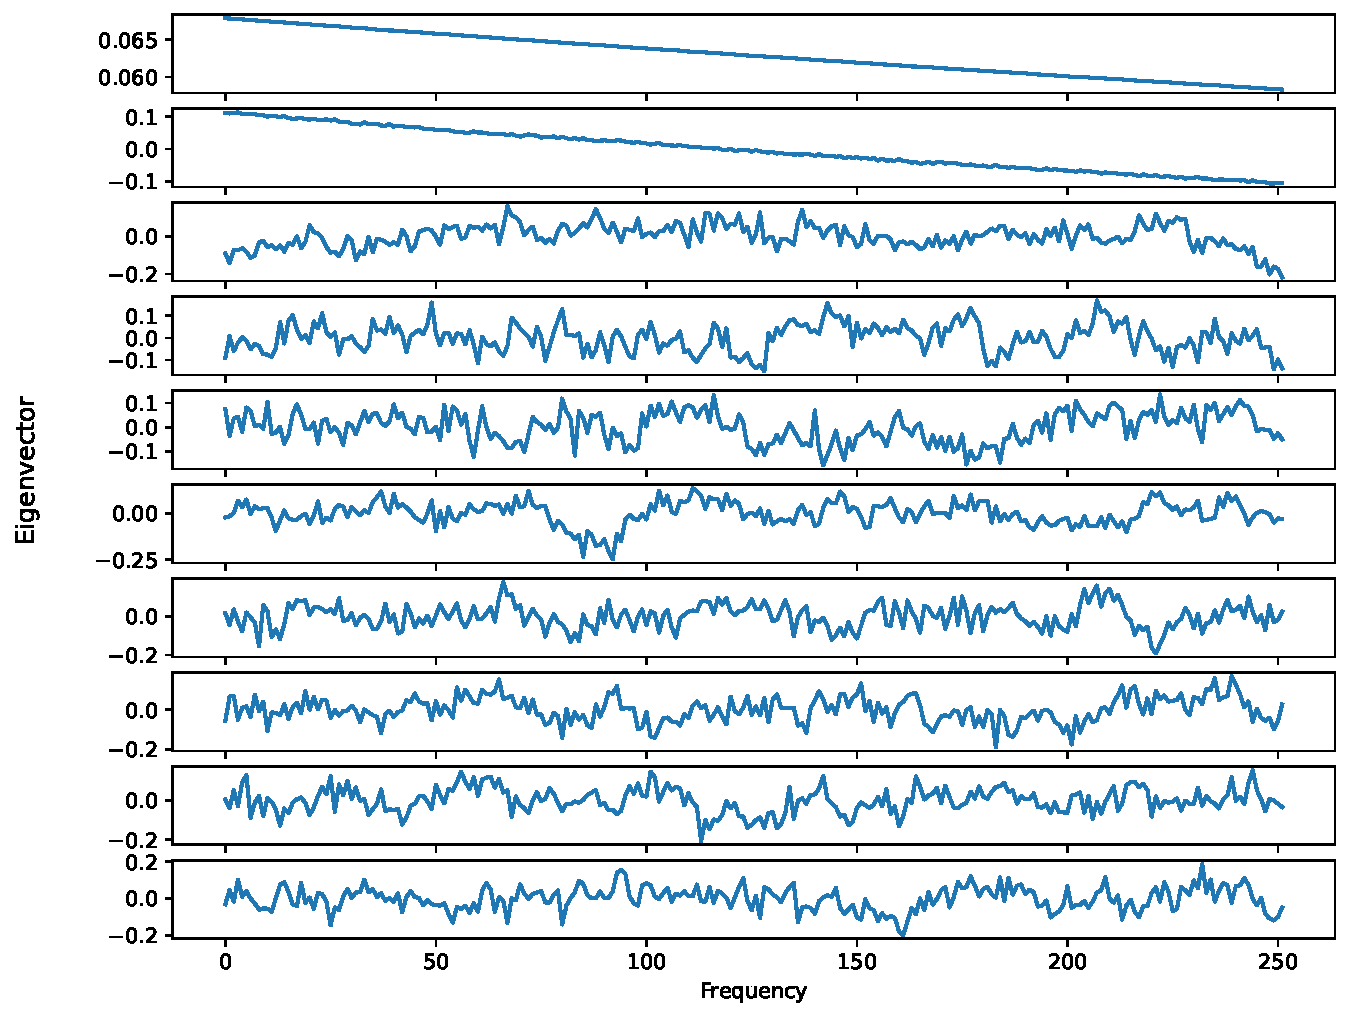
\includegraphics[width=0.7\linewidth]{outputs/week4/eigenvectors.pdf}
    \caption{A plot showing the eigenvector modes versus frequency of the mock data with the total signal consisting of the 21\,cm signal and foreground.}
    \label{fig:eigenvectors}
\end{figure*}

\begin{figure*}[h!]
    \centering
    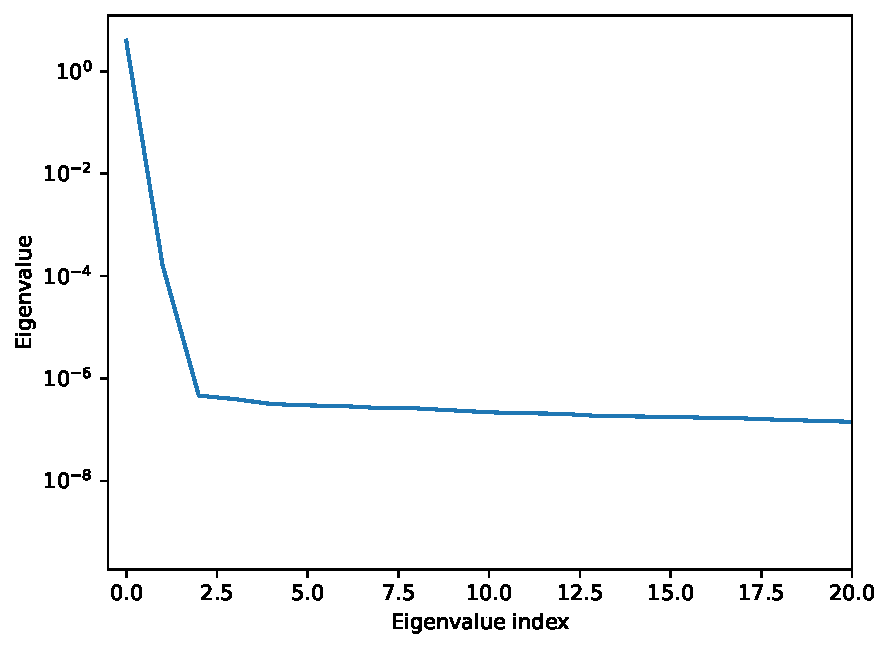
\includegraphics[width=0.65\linewidth]{outputs/week4/eigenvalues.pdf}
    \caption{A plot showing the eigenvalues versus eigenvalue index of the mock data with the total signal consisting of the 21\,cm signal and foreground.}
    \label{fig:eigenvalues}
\end{figure*}

\begin{figure*}[t!]
    \centering
    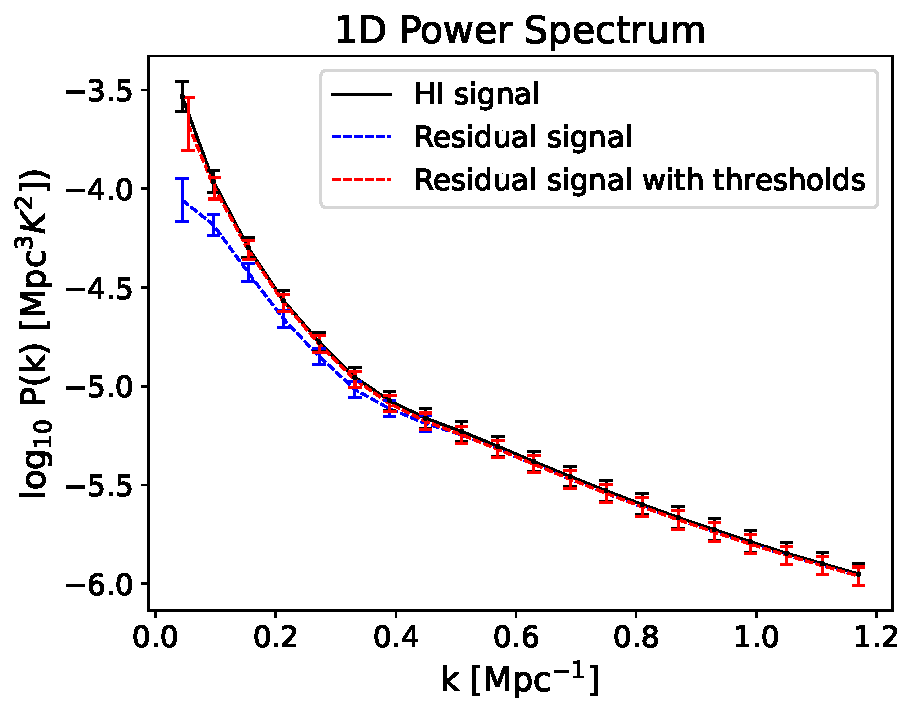
\includegraphics[width=1\linewidth]{outputs/week9/1d_log_power_spectrum_[0, 0.03]_None_both.pdf}
    \caption{The mean cylindrical power spectra of 100 independent realisation from for the HI signal, the PCA residual total signal (HI signal and foreground) after foreground removal, and the ratio between the PCA residual signal and the HI signal, from left to right.}
    \label{fig:cylindrical_power_spectrum_None_None}
\end{figure*}

% [1] https://arxiv.org/pdf/2206.01579
% [2] https://link.springer.com/book/10.1007/b98835 (last sentence but not cited yet)
Principal Component Analysis (PCA) is a blind foreground removal method which requires no prior knowledge of the foreground. This technique takes advantage of the foreground being several orders of magnitude larger than the 21\,cm signal and having a highly correlated frequency structure (\cite{cunningtonHIIntensityMapping2022}).

The data can be described as a matrix $d$ which is a linear system with dimensions $N_\theta \times N_\nu$:

\begin{equation}
    \label{eq:data}
    d = As + d_{clean},
\end{equation}

where $A$ is the mixing matrix and $s$ are the $N_{fg}$ separable foreground components identified by projecting the mixing matrix along the data ${s = A^Td}$. The mixing matrix is extracted from the eigen-decomposition of the frequency covariance matrix of the mean-centred data. This frequency-frequency matrix is defined by 

\begin{equation}
    C = \frac{(wd)^T(wd)}{N_\theta-1},
\end{equation}

where $w$ are the inverse variance weights recast into $N_\theta \times N_\nu$ matrices. The eigen-decomposition of the covariance matrix is given as

\begin{equation}
    C = V\Lambda V^T,
\end{equation}

where $V$ are the eigenvectors ordered by decreasing eigenvalue, and $\Lambda$ is the diagonal matrix of eigenvalues. The first eigenvectors, associated with the largest eigenvalues, correspond to the modes of greatest variance and are dominated by the spectrally smooth foreground emission $N_{fg}$. The first $N_{fg}$ eigenvectors supply the columns of the mixing matrix $A$, since the foreground dominates the largest variance modes. The foreground estimate $As$ can therefore be written explicitly in terms of the eigenvectors as

\begin{equation}
    As = \sum_{n=1}^{N_{fg}}v_nv_n^Td
\end{equation}

where $v_n$ are the foreground eigenvectors being projected out. By substituting this into \Cref{eq:data}, rearranging for $d_{clean}$ gives the foreground-cleaned data: 

\begin{equation}
    d_{clean} = d - As = (I - \sum_{n=1}^{N_{fg}}v_nv_n^T)d,
\end{equation}

where $I$ is the identity matrix. The underlying assumption is that the foreground emission dominates the largest variance modes, so projecting them out leaves a residual signal dominated by the 21\,cm contribution. 

%While effective, this foreground cleaning can also remove some HI signal modes which overlap with the foreground, or leave behind some residual foreground contamination in the cleaned data.

A key strength of PCA is that is requires no prior knowledge of the foreground and it is entirely data driven. It is also computationally efficient, requiring only a single eigendecomposition of the covariance matrix.

However, PCA has two inherent limitations. First, it is a blind method, which means it cannot distinguish between foreground and HI signal modes that share similar spectral structure. At low $k_{\parallel}$, where the HI signal has long frequency correlation scales comparable to the foreground, PCA inevitably removes some genuine cosmological signal alongside the foreground modes. Second, the choice of $N_{FG}$ is not uniquely determined by the data and requires a judgement based on the eigenvalue spectrum. An insufficient number of components leaves residual foreground, while too many risk subtracting genuine HI signal. More rigorous approaches such as cross-validation or Bayesian model selection could determine $N_{FG}$ more objectively. 

\subsubsection{Foreground Removal}

A HI intensity map was generated for a total signal consisting of the 21\,cm signal and the foregrounds. In order to prevent the results being subject to cosmic variance and to quantify the statistical uncertainty on the recovered power spectrum, the foreground cleaning procedure was repeated across 100 independent realisations of the mock data, generated by varying the random seeds used in the simulation. Each realisation produces a different but statistically equivalent realisation of the HI signal, and the spread across realisations reflects the sample variance inherent to a single survey volume. The mean and standard deviation of the data across all realisations were used for plotting the power spectra. This approach provides a more robust assessment of PCA performance than a single realisation alone and allows the consistency of the foreground removal method to be evaluated across different signal realisations.

The eigenvectors and eigenvalues of the total signal covariance are shown in \Cref{fig:eigenvectors} and \Cref{fig:eigenvalues}. The first two eigenvectors are visibly spectrally smooth, consistent with the expected frequency structure of synchrotron and free-free foreground emission. The remaining eigenvectors exhibit rapid frequency oscillations characteristic of the 21\,cm signal and noise. The eigenvalue spectrum shows a sharp drop of approximately 10-11 orders of magnitude after the third eigenvalue, after which the spectrum plateaus at a much lower level. This separation provides justification for the choice of $N_{FG} = 3$, as the first three modes capture the foreground-dominated variance while the remaining modes are consistent with the HI signal. This break in the eigenvalue spectrum is the key diagnostic used to select $N_{FG}$.

%The first few eigenvectors are spectrally smooth, exhibiting the smooth characteristic expected from the foreground. Additionally, the first three eigenvalue modes are the largest and correspond to the foreground. Therefore, $N_{FG} = 3$ principal components were removed from the total signal to perform the foreground cleaning. This value was chosen to maximise foreground suppression while minimising the loss of the HI signal. 

%To recover the desired cosmological information, the equation is rearrange to isolate the residuals: 

%\begin{equation}
%    \epsilon = \textbf{d} - \textbf{As}.
%\end{equation}

\subsubsection{Cylindrical Power Spectrum}

To evaluate the foreground removal, the true HI power spectrum, the residual signal, and their ratio were plotted, seen in \Cref{fig:cylindrical_power_spectrum_None_None}. By inspecting the ratio panel, the components of the wave-vector experiencing signal loss were identified. For the majority of the panel the pixels are red, indicating a ratio of unity, which means that the HI power spectrum has successfully been recovered. However, at low $k_{\parallel}$ and $k_{\perp}$, this ratio goes below unity, revealing signal loss. 

By inspection of where the blue pixels were, an initial minimum threshold of $k_{\parallel} = 0.025$\,Mpc$^{-1}$ and $k_{\perp} = 0.1$\,Mpc$^{-1}$ was tested, followed by different paris of values. The aim was to find the pair of values for $k_{\parallel}$ and $k_{\perp}$ which balanced removing enough foreground without causing too much HI signal loss. Once the optimal threshold was found, foreground cleaning was performed again using the optimal minimum thresholds of wavenumber components, the 1D power spectrum was extracted again and compared to theory.


\subsection{Gaussian Process Regression}

% [1] https://link.springer.com/chapter/10.1007/978-3-540-28650-9_4
% [2] https://mc-stan.org/docs/2_38/stan-users-guide/gaussian-processes.html#:~:text=Unlike%20a%20simple%20multivariate%20normal,mean%20function%20and%20covariance%20function.
In Gaussian Process Regression (GPR), the various components of the signal, which are the foreground and 21\,cm signal, are modelled as realisations of a Gaussian Process (GP; \cite{rasmussenGaussianProcessesMachine2008}). A GP is a Gaussian distribution extended to infinite dimensions. While a standard multivariate Gaussian distribution describes a finite set of variables, a GP expands this to an infinite number of variables. In this context, instead of describing discrete points, the distribution describes continuous functions over a range of frequencies $\nu$. Consequently, a GP provides a probability distribution over a space of possible functions. 

In contrast to multivariate Gaussian distributions, which are defined by a mean vector and covariance matrix, a GP is defined by a mean function and a covariance function. The covariance function is defined by a kernel, which determines the relationship between different points in the data and specifies which functions are likely under the GP prior. This determines the generalisation properties of the model.

%In contrast to multivariate Gaussian distributions, which is defined by a mean vector and covariance matrix, a GP is defined by a mean function and a covariance function. In this case, each element of the mean is a function of frequency and the covariance function is defined by a kernel which means they are easy to sample from. A kernel, also known as a covariance function or kernel function, defines the shape of the functions by determining the relationship between different points in the data and is the set of functions considered for the data. It specifies which functions are likely under the GP prior. This, then, determines the generalisation properties of the model.

GPR operates in a similar way to regression with parametric models, with the main distinction being that a prior is put on the the kernel rather than on the specific model coefficients, where conventionally the prior has a mean of zero. GPR is a non-parametric regression technique, meaning it is able to estimate relationships between variables without assuming a predefined function form. Instead, the model is constructed directly from the data, making it useful for complex, unknown, or non-linear datasets. 

% [3] https://arxiv.org/pdf/2102.01697
Another advantage of GPs is that it is stochastic, which mean that each realisation is random and can take any functional form consistent with the mean and kernel function. Assuming only Gaussian noise is present, they also have a well defined marginal likelihood function, so it is easy to compute the probability of data conditioned on a given value of the mean and kernel functions (\cite{lugerMappingStellarSurfaces2021}). %This can be maximised to find the optimal values of the model parameters or be used to evaluate the posterior which is very useful for inference problems.

However, GPs require a larger amount of data to achieve the same level of uncertainty as a parametric model, pose a higher risk of overfitting, are slower to compute, and can be difficult to interpret.

The assumption is made that the data, and each of its components, are drawn from a GP with a kernel function and zero mean, which is consistent with the data being mean-centred. Since the total data is composed of separate GP components, the total kernel can be decomposed as

\begin{equation}
    K_{tot} = K_{fg}+K_{HI},
\end{equation}

where $K_{fg}$ and $K_{HI}$ are the foreground and HI kernels respectively.

Given this decomposition, the GP conditional mean provides the optimal estimate of the foreground signal given the total observed data. The foreground contribution is estimated as

\begin{equation}
    \hat{f} = K_{fg}(K_{fg}+K_{HI})^{-1}d.
\end{equation}

The cleaned residual map is then obtained by subtracting this estimate from the total data:

\begin{equation}
    d_{clean} = d - \hat{f} = [I - K_{fg}(K_{fg}+K_{HI})^{-1}]d
\end{equation}

\begin{equation}
    d_{clean} = K_{HI}(K_{fg}+K_{HI})^{-1}d
\end{equation}

The cleaned map retains only the component of the data best explained by the HI kernel, with the foreground contribution projected out. The quality of this cleaning therefore depends critically on how well the fitted kernels describe the true covariance structures of each component.

%Since the data is made up of separate components which are all GPs, the kernel function can also be split into separate components: the foreground kernel and the 21\,cm signal kernel. Since the foreground model is a GP, it has an expectation value and covariance. The expectation value is a prediction of the foreground signal and is dependent on both the foreground kernel, the total kernel of the data, and the data. While, the covariance provides information on the uncertainty on this prediction. Therefore, it is important there are suitable kernels for all components of the data. 

%By making an educated estimate of the true foreground signal with an appropriate kernel, the foreground signal can be modelled. This can be removed from the data, by subtracting the expectation value of the foreground from the data, and the residual signal, ideally left with the instrumental noise the the desired 21\,cm signal, is achieved. 

\subsubsection{Kernel functions}

% [1] https://www.cs.toronto.edu/~duvenaud/cookbook/
% [2] https://www.repository.cam.ac.uk/items/a54f0711-f777-4ee1-a685-3b76dae5ad91
% [3] https://gaussianprocess.org/gpml/chapters/RW.pdf
The selection of kernel functions is critical as it significantly affects the generalisation properties of the GP model. The choice of kernel functions is data driven, as they must be chosen to best describe the covariance of the data, along with the best-fitting hyperparameters, which are the parameters of the kernel functions. One commonly used function is the Matern kernel (\cite{rasmussenGaussianProcessesMachine2008}):

\begin{equation}
    K(\nu, \nu') = \sigma^2 \frac{2^{1-\eta}}{\Gamma(\eta)}(\sqrt{2\eta}\frac{|\nu - \nu'|}{l})^\eta K_\eta (\sqrt{2\eta}\frac{|\nu - \nu'|}{l}),
\end{equation}

where $\Gamma$ is the gamma function, $K_\eta$ is the modified Bessel function. This kernel has three hyperparameters which be need to optimised:

\begin{itemize}
    \item \textbf{Variance $\sigma^2$:} this describes the amplitude or "power" of the signal. Since the foregrounds are significantly brighter than the HI signal, $\sigma^2$ is expected to be much larger for the foreground component (see \Cref{fig:frequency_vs_temperature}).
    \item \textbf{Lengthscale $l$:} this describes the scale of frequency correlations. A larger $l$ indicates the data points are more correlated over wide frequency ranges. A larger lengthscale is expected for foregrounds since they are much more correlated in frequency (see \Cref{fig:tot_fg_hi_noise_covariance}).
    \item \textbf{Spectral parameter $\eta$:} this determines the smoothness of the function. Since the foregrounds are smooth in frequency and the HI signal is more Gaussian, $\eta$ is expected to be larger for the foregrounds than for the HI signal (see \Cref{fig:frequency_vs_temperature}).
\end{itemize}

By choosing different values for the spectral parameter $\eta$, the Mat\'ern kernel can simplify. This project will use two choices for this hyperparameter:

% [4] https://arxiv.org/abs/2010.15892
% [5] https://academic.oup.com/mnras/article/493/2/1662/5727337#sec3
% [6] https://arxiv.org/pdf/2105.12665
% [7] https://academic.oup.com/mnras/article/478/3/3640/4995230
\begin{itemize}

    \item \textbf{$\eta \rightarrow \infty$:} the Mat\'ern kernel simplifies to the Radial Basis Function (RBF), also known as the squared exponential or Gaussian kernel. This represents an extremely smooth signal which makes it the ideal choice for modelling the foreground component. \cite{kernGaussianProcessForeground2020}, \cite{mertensImprovedUpperLimits2020} and \cite{soaresGaussianProcessRegression2022} use this kernel to model their smooth foreground component. This has the form:

    \begin{equation}
        \label{eq:RBF}
        K(\nu, \nu') = \sigma^2 exp(\frac{(\nu - \nu')^2}{2l^2}).
    \end{equation}

     %\item \textbf{$\eta = 5/2$:} the Matern kernel is not quite as smooth in frequnecy as the RBF kernel but is still relatively smooth. This kernel was used to model the smooth foreground component by [7].
    
    %\item \textbf{$\eta = 3/2$:} the Matern kernel is even less smooth in frequency and can be used to describe foreground components with moderate frequency smoothness. This was done by \cite{mertensImprovedUpperLimits2020} and [7].
    
    \item \textbf{$\eta = 1/2$:} the Mat\'ern kernel is the least smooth in frequency and simplifies to the exponential function. Since it is not smooth at all, it is a strong match for signals that vary significantly with frequency, such as the HI signal. This is used to describe the HI signal by \cite{kernGaussianProcessForeground2020}, \cite{mertensImprovedUpperLimits2020}, and \cite{soaresGaussianProcessRegression2022} and has the form: 

    \begin{equation}
        \label{eq:exp}
        K(\nu, \nu') = \sigma^2exp(\frac{|\nu - \nu'|}{l}).
    \end{equation}
    
\end{itemize}

The versatility of the Mat\'ern kernel makes it a strong tool for various signals. By adjusting its hyperparameters, each component of the data can be effectively modelled.

\begin{figure}[t!]
    \centering
    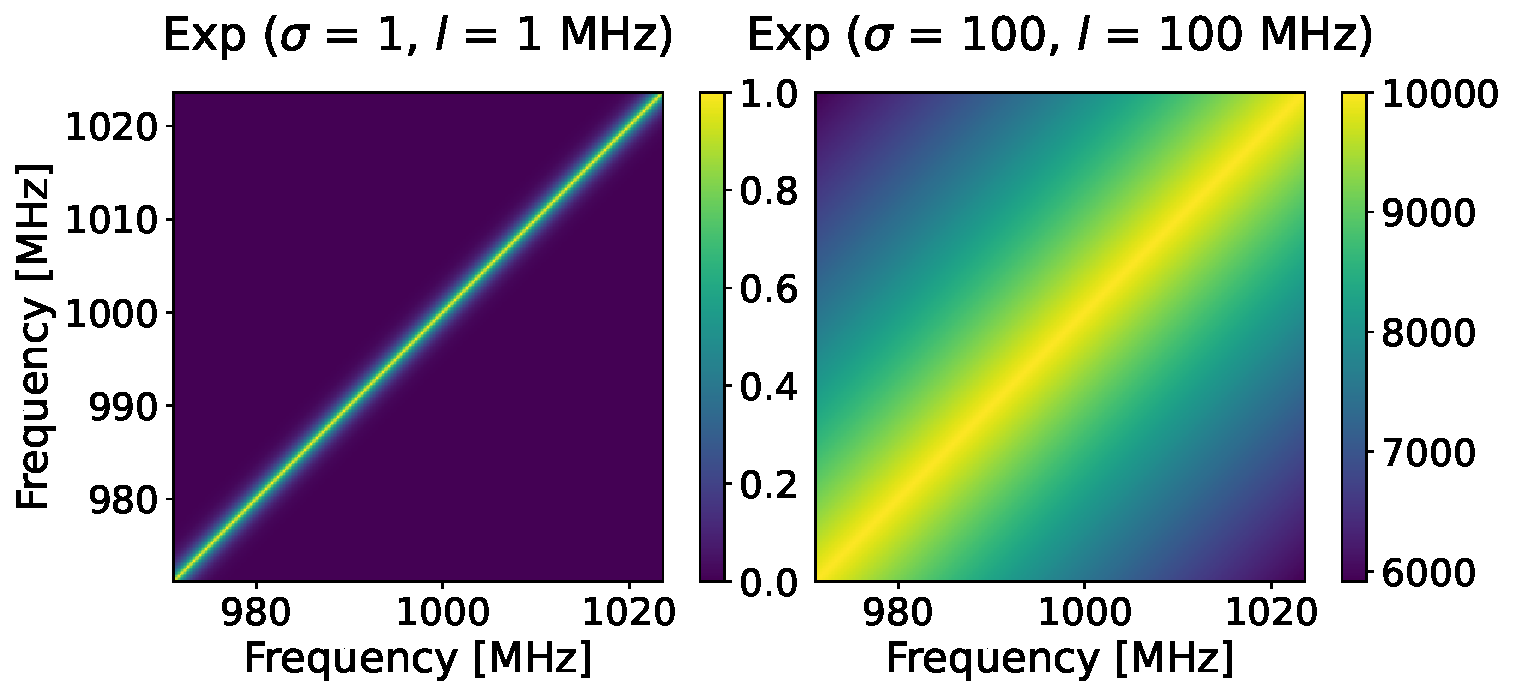
\includegraphics[width=1\linewidth]{outputs/week6/exp_kernel_lengthscales_2.pdf}
    \caption{Frequency covariance of the exponential kernel with a low variance and low lengthscale ($\sigma = 1$, $l = 1$) seen on the left, and another with a high variance and high lengthscale ($\sigma = 100$, $l = 100$) seen on the right. This exponential kernel is used to model the 21\,cm cosmological signal.}
    \label{fig:exp_kernel_lengthscales}
\end{figure}

\begin{figure}[t!]
    \centering
    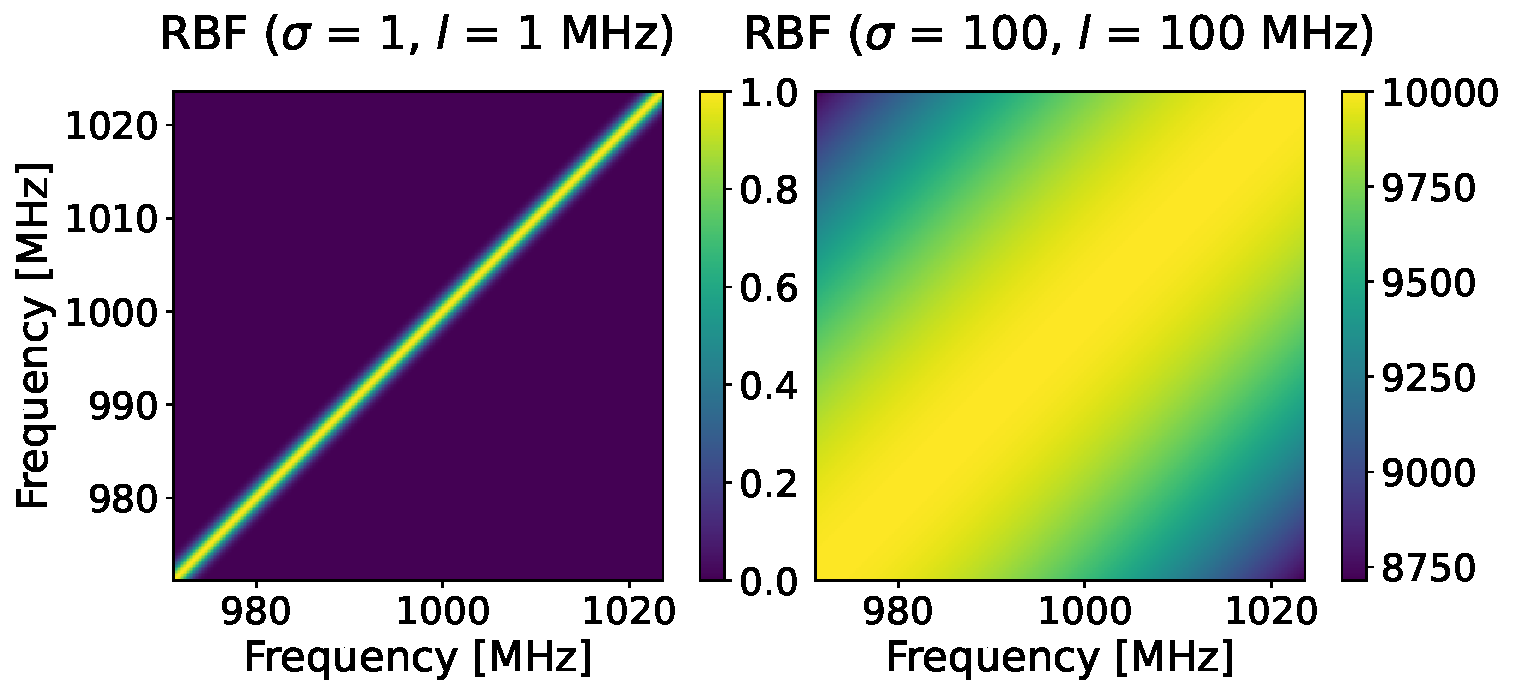
\includegraphics[width=1\linewidth]{outputs/week6/rbf_kernels_lengthscales_2.pdf}
    \caption{Frequency covariance of the radial-basis function (RBF) kernel with a low variance and low lengthscale ($\sigma = 1$, $l = 1$) seen on the left, and another with a high variance and high lengthscale ($\sigma = 100$, $l = 100$) seen on the right.}
    \label{fig:rbf_kernels_lengthscales}
\end{figure}

\begin{figure}[t!]
    \centering
    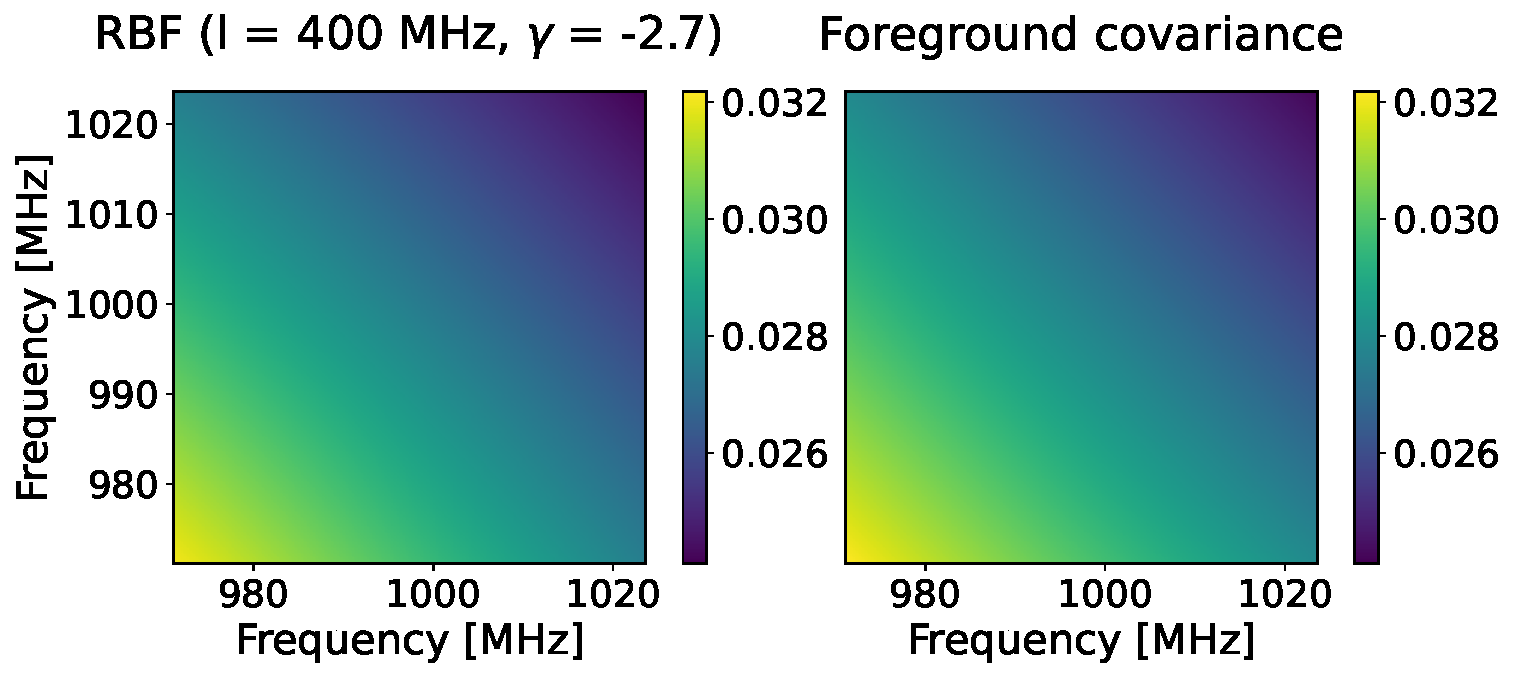
\includegraphics[width=1\linewidth]{outputs/week6/rbf_kernel_w_sp_indx_vs_foreground_covariance.pdf}
    \caption{Frequency covariance of the spectral index modified radial-basis function (RBF) kernel with high lengthscale and a spectral index ($l = 400$, $\gamma=-2.7$) seen on the left, and the true foreground covariance seen on the right. This spectral index modified RBF kernel is used to model the foreground signal.}
    \label{fig:rbf_kernel_w_sp_indx_vs_foreground_covariance}
\end{figure}

To demonstrate the behaviour of the exponential and RBF kernels, both are presented in two cases: one with a low variance and low lengthscale ($\sigma = 1$, $l = 1$), and another with a high variance and high lengthscale ($\sigma = 100$, $l = 100$), shown in \Cref{fig:exp_kernel_lengthscales} and \Cref{fig:rbf_kernels_lengthscales}. Increasing $l$ broadens the diagonal stripe, raising the correlation of the signal. Increasing $\sigma$ raises the amplitude of the covariance. By comparing these plots to the true covariance structures (\Cref{fig:tot_fg_hi_noise_covariance}), it is clear that the exponential kernel with small $\sigma$ and $l$ best describes the HI signal, while the RBF kernel with large $\sigma$ and $l$ best describes the foreground.

However, the standard RBF kernel has diagonal symmetry not seen in the true foreground covariance. To better reproduce the foreground's frequency-dependent amplitude scaling, which is physically motivated by the power-law spectrum of the synchrotron emission, a spectral index parameter $\gamma$ is introduced such that 

%We can see that the RBF function has a much wider diagonal in both cases. A wider diagonal means that the data is much more correlated in frequency. A smaller diagonal means that the data points are less correlated in frequency and are mainly correlated with themselves and the points directly around them. 

%By inspection, we can tell that the exponential kernel function with low $\sigma$ and low $l$ would be the best fit for the 21\,cm signal while the RBF function with a high $\sigma$ and high $l$ would best fit the foreground component. However, while the amplitude of the RBF covariance matches that of the foreground, the RBF covariance has diagonal symmetry that is not seen in the foreground. In order for the shape of the RBF function to match this foreground signal better, we can add a spectral index parameter $\gamma$ so the signal can scale according to frequency 

\begin{equation*}
    T(f) = T_0(f_0) * (\frac{f}{f_0}) ^ \gamma.
\end{equation*}

This modifies the RBF kernel to

\begin{equation}
    \label{eq:RBF_sp_indx}
    K(\nu, \nu') = \sigma^2 exp(\frac{(\nu - \nu')^2}{2l^2})(\frac{\nu}{\nu_0})^\gamma(\frac{\nu'}{\nu'_0})^\gamma,
\end{equation}

where $\nu_0$ and $\nu'_0$ are the first frequency values in the range. While previous studies including \cite{kernGaussianProcessForeground2020}, \cite{mertensImprovedUpperLimits2020}, and \cite{soaresGaussianProcessRegression2022} use the standard RBF kernel for foreground modelling, this work uses the spectral-index-modified form of \Cref{eq:RBF_sp_indx}, allowing the foreground amplitude to vary with frequency in a physically motivated way. The application of this modification can be seen in \Cref{fig:rbf_kernel_w_sp_indx_vs_foreground_covariance}, where the spectral-index-modified RBF kernel better reproduces the gradient structure of the true foreground covariance.

%The application of this can be seen in \Cref{fig:rbf_kernel_w_sp_indx_vs_foreground_covariance} where we can see that this addition for the RBF kernel to mimic the reality that the foregrounds are much brighter at lower frequencies. 

% [1] https://arxiv.org/pdf/2105.12665
%The goal is to find the kernel functions which best mimic the different components of the data which are the foreground and 21\,cm signal. 

%There are a couple of ways to handle noise in GPR. Since the noise is so small in amplitude and so highly correlated in frequency, it can be treated as indistinguishable noise as done by \cite{soaresGaussianProcessRegression2022}. This assumes there is either no noise present in the data, or the noise is indistinguishable from the other signals which means that the covariance functions of the other signals describes and captures the noise. It is important to noise that this data is idealised and real data would likely results in much more complex instrumental noise which would require a more rigorous treatment.

\subsubsection{Hyperparameter optimisation and model selection}

Model selection for GPR is a two step process. The first step is to choose the kernel function that best models the data, and the second is to optimise the hyperparameters. This is done with a Bayesian approach by computing the marginal likelihood and selecting the model that maximises it. 

%This represents the probability of the data given some hyperparameters $\theta$. By integrating the likelihood $\mathcal{L}$ multiplied by the prior over the GP realisations, the Log-Marginal Likelihood (LML) can be obtained: 

%It is important to pick the kernel function which performs the best along with their most optimal hyperparameters that best model the signals. These two steps are mutually dependent. So, although we have found kernel function which match our data by inspection, we much compare the overall performance of each model. This will be done by first optimising the hyperparameters of each kernels by maximising their marginal likelihoods. This will then be compared to other optimised kernel functions. 

%To evaluate each model, the marginal likelihood, also known as the Bayesian evidence, was computed. This represents the probability of the data given some hyperparameters $\theta$. By integrating the likelihood $\mathcal{L}$ multiplied by the prior over the GP realisations $x$, the Log-Marginal Likelihood (LML) can be obtained: 

%For a kernel function with hyperparameters $\theta$, the marginal likelihood of the data can be calculated by integrating the data likelihood $\mathcal{L}$ multiplied by the prior. 

%\begin{equation}
%    p(d|\nu, \theta) = \int \mathcal{L}(d|x, \nu, \theta) p(x|\nu, \theta) dx
%\end{equation}

\begin{equation}
    \log p(d|\nu, \theta) = -\frac{1}{2} tr(CK^{-1}) - \frac{1}{2} \log|K|
\end{equation}

where $C$ is the observed frequency-frequency covariance matrix of the data, $K=K_{HI}+K_{fg}$ is the total kernel function, and $\theta$ is the set of hyperparameters. This covariance-based form is used rather than standard data-vector form because the foreground removal is performed in covariance space, which fits the kernel model to the observed covariance structure of the total signal rather than to individual data realisations. The LML can be computed analytically since each component of the data is assumed to be a GP.

To compare different kernel models, the log Bayes factor $\mathcal{Z}$ is computed as the difference in LML between two models: 

\begin{equation}
    \log \mathcal{Z} = LML_{method_1} - LML_{method_2}
\end{equation}

where a larger value of $\mathcal{Z}$ or $\log \mathcal{Z}$ means that the first model fits the data better than the second model.

% [1] https://academic.oup.com/mnras/article/493/2/1662/5727337#199912059
% [2] https://arxiv.org/pdf/2105.12665
In practice, the optimal hyperparameters can be found using standard optimisation, Monte Carlo Markov Chain (MCMC) methods as used by \cite{mertensImprovedUpperLimits2020}, or Nested Sampling as used by \cite{soaresGaussianProcessRegression2022}. Standard optimisation is computationally inexpensive but is prone to converging in local minima and provides no uncertainty estimates. Nested Sampling is designed to compute the marginal likelihood directly and handles multimodal posteriors well, but is highly computationally expensive. MCMC provides a full posterior distribution over parameters, is better at exploring the global parameter space, and is computationally intermediate between the two methods.

%On the other hand, Nested Sampling is designed specifically to calculate the marginal likelihood and is good at handling data with several separate peaks with high likelihoods. This, however, is highly complex and much more computationally expensive. MCMC Sampling provide a full posterior showing the probability distribution and correlation between parameters. They are also better at finding the global peak as it explores parameter space. This method takes much longer than standard optimisation techniques but runs quicker than Nested Sampling, thus, being a middle ground between the two methods. 

% [1] https://ui.adsabs.harvard.edu/abs/2013PASP..125..306F/abstract
In this work, the SciPy minimize function (\cite{virtanenSciPy10Fundamental2020}) was used for initial hyperparameter optimisation to efficiently compare LMLs across different combinations of algorithms, hyperparameter initial guesses, and bounds. The LMLs obtained from this initial optimisation were compared across kernel combinations to identify the best-fitting model, which was then used for MCMC sampling using the \texttt{emcee} package (\cite{foreman-mackeyEmceeMCMCHammer2013a}).

Initial guesses for the optimisation were chosen by visual comparison of the kernel functions to the true covariance structures. For example, the 21\,cm signal is tightly correlated along the diagonal (see \Cref{fig:tot_fg_hi_noise_covariance}), suggesting small $l$ and small $\sigma$ with the exponential kernel. The foreground is smooth and high-amplitude, suggesting large $l$, large $\sigma$, and a negative spectral index with the RBF kernel. Bounds were set to exclude unphysical values. For example, the spectral index was constrained to be negative, consistent with the observed decrease in synchrotron brightness with increasing frequency.

%Initial guesses must be provided for the algorithm to start on. These intial guesses are important as the algorithm is sensitive to this and an incorrect starting point may result in a final value which is unphysical. These initial guesses were taken by fitting different values of the lengthscale $l$ and variance $\sigma$ to the kernels to try to mimic the true covariance of the signal components. For example, we know the 21\,cm signal is very tightly and strongly correlated in frequency (see \Cref{fig:tot_fg_hi_noise_covariance}) so a smaller $l$ and smaller $\sigma$ would be suitable with the exponential kernel (see \Cref{fig:exp_kernel_lengthscales}). On the other hand, the foreground is very smooth in frequency and high in amplitude (see \Cref{fig:tot_fg_hi_noise_covariance}) so the RBF kernel with high $l$, high $\sigma$ and a spectral index would be most suitable (see \Cref{fig:rbf_kernel_w_sp_indx_vs_foreground_covariance}).

%In addition to this, bounds must be set for each of the hyperparameters for both of these methods. This means that the algorithms will not explore any values that are unphysical. Again, these are chosen of what would be appropriate by inspection of the kernel functions and with knowledge of the data. For example, we know that the spectral index must be negative otherwise the amplitude would increase with frequency and that is the opposite of what we see. A reasonable range around the initial guesses would be a suitable choice. 

% [2] https://joss.theoj.org/papers/10.21105/joss.00024
The 100 walkers were initialised in a tight Gaussian ball centred on the best-fit hyperparameters from the initial optimisation, with a perturbation of 0.1\% applied to each hyperparameter. A prior check was applied to ensure all walkers began within the defined flat (uniform) prior bounds. Each walker evolved by proposing moves informed by the positions of the other walkers, preferentially sampling regions of high posterior probability while retaining the ability to explore lower-probability regions, avoiding convergence to local maxima. The chains were run for 10,000 steps with the first 1,000 discarded as burn-in. The thinning factor was chosen to be approximately half the autocorrelation time of the chain, ensuring that successive samples are approximately independent. Hence, the chain was thinned by retaining every 40th steps, yielding an approximately independent set of posterior samples. Convergence of the walkers were assessed through the mean acceptance fraction, visual inspection of parameter trace plots, and the corner plots (\cite{foreman-mackeyCornerpyScatterplotMatrices2016a}).

To quantify the uncertainty on the recovered power spectrum arising from the kernel hyperparameters, 1,000 parameter sets were drawn at random from the MCMC posterior chain. From each draw, the corresponding HI and foreground kernels were constructed and foreground cleaning was applied, yielding 1,000 independent realisations of the cleaned map. The 16th, 50th, and 84th percentiles were then computed across these realisations at each $k$, corresponding to the median recovered power spectrum and its 1$\sigma$ interval. These represent the uncertainties on the residual power spectrum, representing how sensitive the foreground removal is to the uncertainty in the fitted kernel parameters. 

The MCMC sampling was performed with a single fixed random seed, meaning that while hyperparameter uncertainties were obtained, cosmic variance was not accounted for. Ideally, the sampling would be repeated across 100 independent realisations of the HI signal, as done with PCA, with uncertainties derived from the resulting spread. However, due to computational and time constraints, this single-seed approach was deemed sufficient for the purposes of this work.